\chapter{Consideration}

While currently both OpenCSD and FluffleFS are complete enough to performance
experimental evaluation several aspects have to be considered that can be
substantially improved. Throughout this sections those aspects are divided into
five categories. Firstly, several limitations in FluffleFS prevent regular use
of the filesystem outside of experimental settings. Secondly, the current
prototype has limited concurrency due to the use locks. Third, this simulation
framework can not be used as practical implementation and we would like to
address the necessary changes. Fourth, as previously mentioned, event kernels
suffer from unnecessary latency and data movement due to waiting for the
outstanding I/O request to complete before the kernel is submitted. To address
this we propose a mechanism for event kernels that allows the regular I/O
request to complete on the device itself. Lastly, we describe several
instruments that can be used for safety regarding user submitted kernels.

\section{Filesystem Limitations}

Firstly, the current filesystem limitations of FluffleFS make it unuseable
outside of experimental applications. Foremost, many of the datastructures are
not routinely flushed to the drive even if \textit{fsync} is called. Among
these datastructures are checkpoints, NAT and SIT blocks as well as some others.
As a result, the filesystem is incapable of restoring the previous state when
remounting a previously created filesystem.

Beyond basic setup and teardown is the inability to perform garbage collection.
Meaning no used drive space can be reclaimed. This prevents FluffleFS from
reaching steady state. The ability to delete files and directories is also
currently missing.

Lastly, since several datastructures are not flushed to the drive some mechanism
to read data from the drive are not in place. For instance \textit{lookup} will
never traverse the \textit{inode\_lba\_map} and instead solely relies on
\textit{path\_inode\_map}. This results in the \textit{path\_inode\_map} not
being used for caching instead containing all paths from all to all files and
directories for the entire fileystem.

While it is important to clearly describe the severe practical shortcomings of
FluffleFS note that all these limitations are resolved in the design. Given the
requirements set out by the experiments and time constraints implementing these
features is left as future work.

\section{Concurrency}

Similarly, the degree of concurrency achieved throughout OpenCSD and FluffleFS
is significantly less then possible with the current design. Both time
constraints and these optimizations not being required for the experiments have
led to the decision to prioritize elsewhere. This section describes several
areas that can easily be improved.

Firstly, every filesystem operation utilizes a global lock. As mentioned
previously this MRSW lock allows some operations to operate concurrently while
providing mutual exclusion for critical operations. However, many of the
operations currently utilize the lock in the mutually exclusive mode (writer)
while this can be avoided if underlying datastructures are better protected.
These include in no particular order \textit{lookup}, \textit{getattr},
\textit{setattr}, \textit{readdir}, \textit{open}, \textit{release},
\textit{create}, \textit{fsync}, \textit{getxattr} and \textit{setxattr}.

With such a predominant amount of the operations being entirely serialized with
respect to one another it is very likely this will hinder performance in a
non-neglible manner. For completeness, the remaining operations include
\textit{read} and \textit{write} as necessary per our design requirements to
achieve concurrent regular and offloaded access.

Beyond the filesystem itself the current NVMe backend also suffers from limited
concurrency. In a similar manner this is due to the use of a global lock that
serializes the incoming \textit{read}, \textit{append} and \textit{reset}
operations together. This current limitation is necessary as currently a single
SPDK queue of 4096 bytes in size is used. However, both SPDK and the underlying
NVMe device are capable of having multiple operations being queued concurrently.
While several limitations apply such as only one pending \textit{append} per
zone\footnotemark[16] it is clear a lot of the underlying drive performance is
unutilized in this manner.

\footnotetext[16]{Although multiple sectors can be written in this single
append, within ZNS this is known as queue depth beyond one.}

Importantly, utilizing multiple pending operations is not the same as supporting
an iodepth beyond one neither is it utilizing ZNS append with a queue depth
beyond one.

Last is UBPF as the current system for scheduling kernels can only support one
instance concurrently. Because of this all calls to start running a new kernel
are serialized using a global lock. This last problem is less trivial to resolve
compared to those previously discussed. Within uBPF an instance of the VM object
needs to be bound to methods as key value pairs. Here each key is a specific
number that is supplied as first argument to the \textit{call} instruction in
the eBPF ISA. However, the signature of these hooked methods is identical as how
it will be exposed to the eBPF kernel. This leaves no state or arguments that
can be passed along to associate the specific instance of uBPF once trapped into
the hooked method.

% Figure of transition between kernel and host with method signature and how
% this can't be associated to correct instance (show 3 as example).

A possible solution would be to pass the instance of uBPF as first argument and
supplying the kernels with the instance of their own VM. This breaks isolation
and has many negative side effects in terms of security as well requiring the
disabling of the memory access verifier.

Instead, each instance of uBPF should be associated with a unique sufficiently
sized hash that is presented to the kernel instead. Upon each \textit{call} this
hash is passed as first argument. Once trapped inside the method this hash is
looked up and matched to its respective instance. Should there be no matching
hash the kernel will immediately be terminated. Given a sufficiently large
hash domain the change of a malicious actor finding a match for any concurrently
running instance of uBPF that is not its own are net zero.

% figure of transistion between kernel and host with hash as first argument and
% reverse lookup inside hash table to find uBPF instance.

Clearly, there are many potential performance improvements related to
concurrency that could benefit the current OpenCSD and FluffleFS prototype.

\section{Design for Manufacter}

Beyond concurrency the current prototype suffers from several design decisions
and implementations details that are not suitable for pracitcal implementations.
Many of these limitations arise from being a monolithic application simulation
the offloading rather than submitting it to an actual embedded device. In this
section the necessary changes to create real world practical implementations are
described.

Firstly, the current proposed changes to the NVMe command set are implemented as
shared library linked at compile time. Such an interface where data can be
easily moved back and forth is not pracitcal for systems utilizing communication
protocols and busses. This interface needs to be redesigned with limitations of
these protocols inmind such as limited request size of individual commands and
the asynchronous nature of command submissions. Luckily many extensions to
the NVMe protocol already exist, ZNS being a notable example.

Secondly, the interface exposed to user submitted eBPF kernels needs to be
formalized. Furtermore, this interface needs to be ratified as part of the NVMe
protocol extension so that the minimum set of supported calls from within 
user submitted kernels is non-optional. This will prevent users from having to
rewrite or recompile kernels across different vendors. Given the limited compute
capabilities typically found on these embedded platforms runtime evaluation of
appropriate interfaces should not be an acceptable solution either.

Third, once the new extension to the NVMe command set is ratified existing
drivers such as SPDK, xNVME or those found in the Linux kernel need to be
updated to support this. Likely both the driver and the firmware on the device
will be responsible for scheduling of submitted kernels. Some ideas on this are
detailed while discussing \textit{filesystem agnostic kernels} but no complete
scheduling solution is presented in this work.

Finally, we show an example of the complete data path across all components as
described in this section in figure \ref{figure:practicalarchitecture}.

\begin{figure}
    \centering
	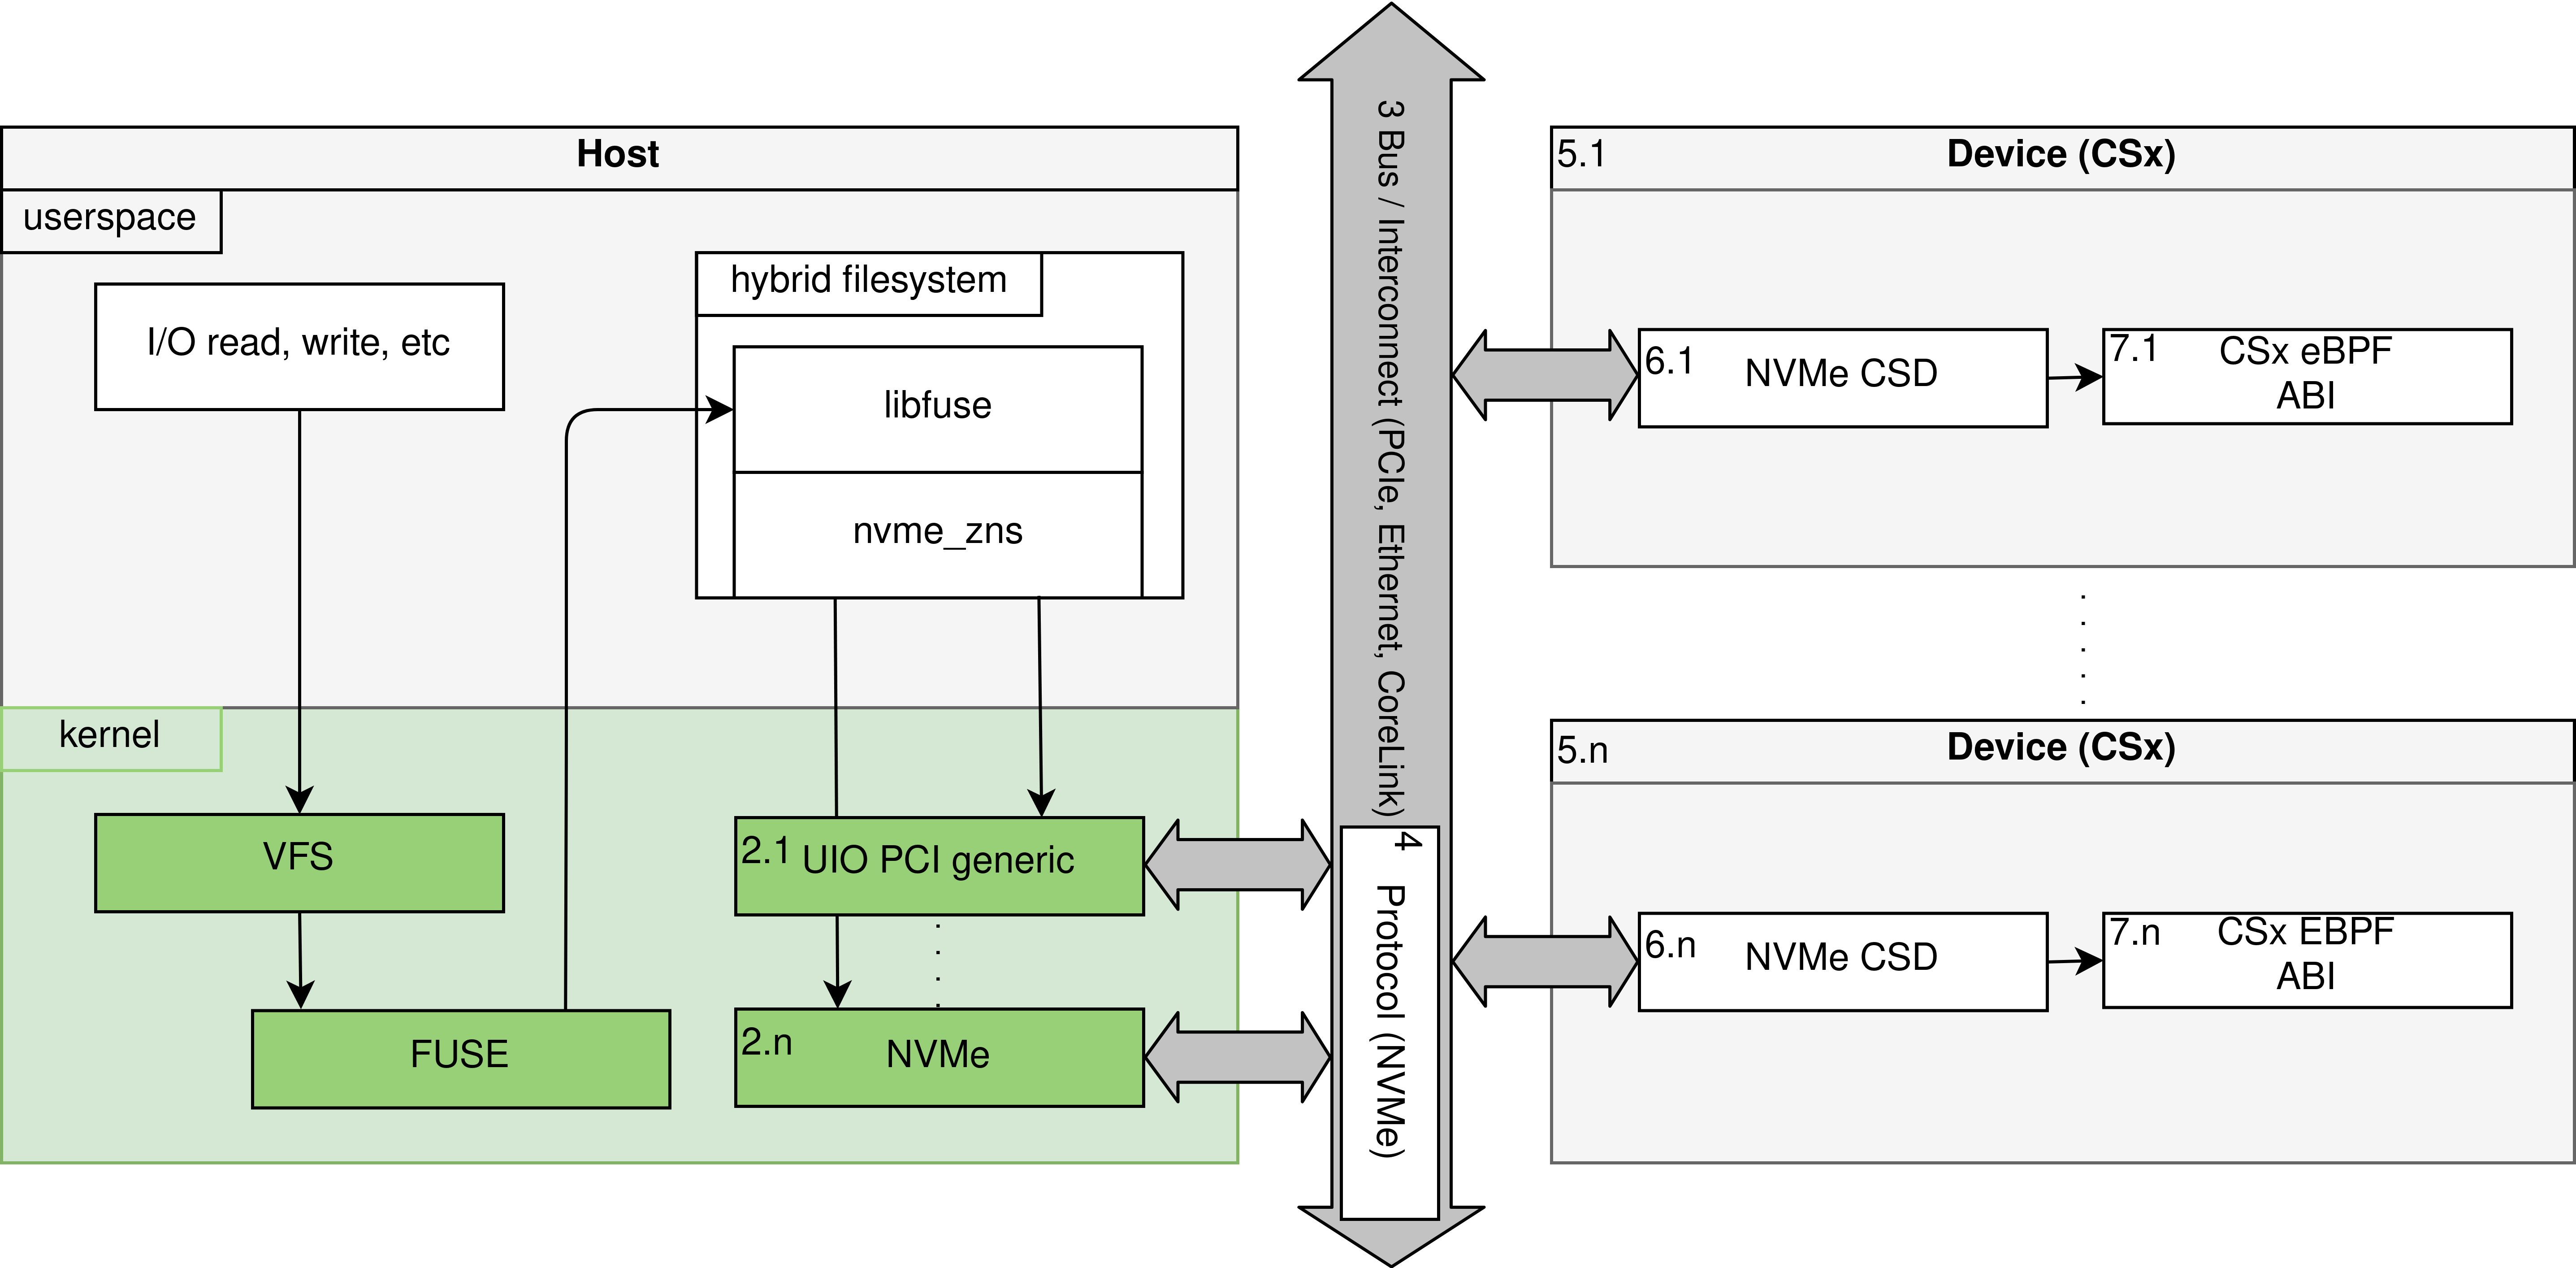
\includegraphics[width=1\textwidth]{resources/images/loader-pfs-arch-v3.png}
	\caption{Practical complete architecture for vendor agnostic CSxs with
        potential filesystem support.}
    % \includesvg[width=0.6\columnwidth]{resources/images/module-dependencies}
    \label{figure:practicalarchitecture}
\end{figure}

\section{Effective Event Kernels}

As mentioned the current event kernel implemenation suffers from unnecessary
data movement and latency. To demonstrate this situation the data path across
requests to and from the CSx is shown in figure
\ref{figure:currenteventkernels}. In this figure the process of opening the file
and setting the extended attribute has been omitted.

\begin{figure}
    \centering
	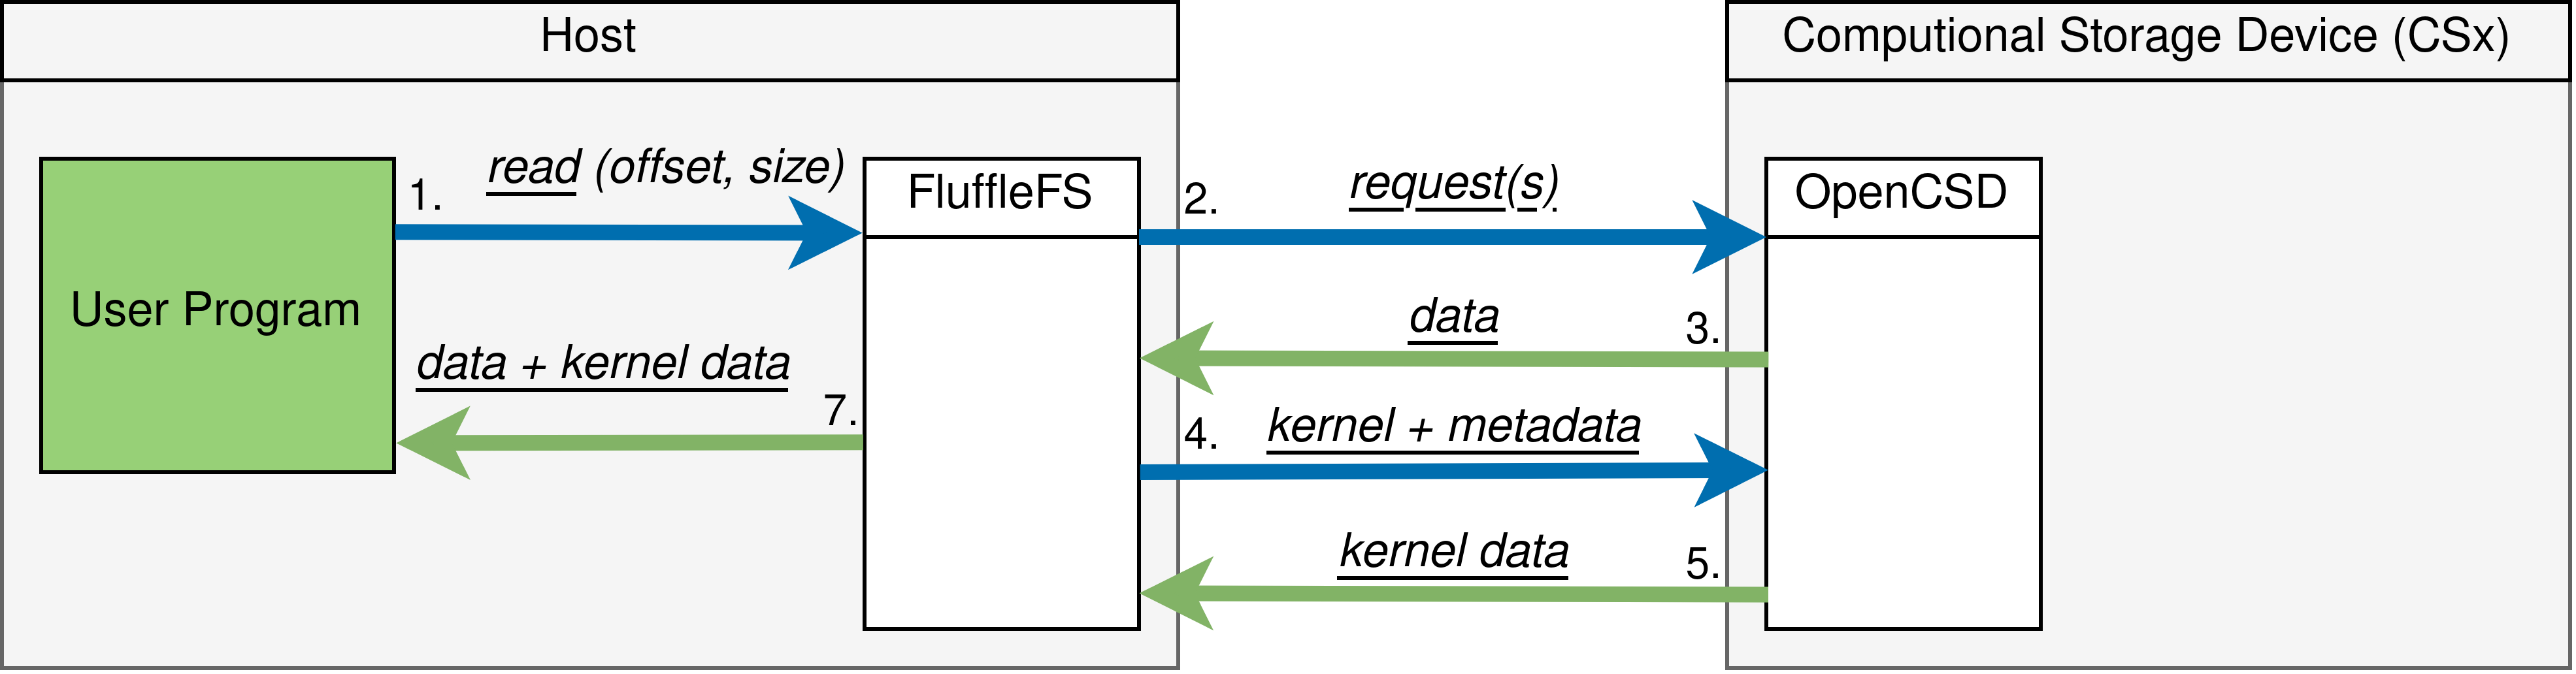
\includegraphics[width=1\textwidth]{resources/images/current-event-kernel.png}
	\caption{Current implementation of event kernels.}
    % \includesvg[width=0.6\columnwidth]{resources/images/module-dependencies}
    \label{figure:currenteventkernels}
\end{figure}

As shown the filesystem sends the request along to the drive after receiving the
read request from the user. After receiving this data in step three the
filesystem can now submit the user kernel along with the necessary metadata to
the CSx. Finally, after the kernels completion the combined data can be returned
to the user. The procedure is identical for write requests except no data is
returned to the host upon completion of the request and the kernel.

In order to reduce the latency and unnecessary data movement we propose a
multistage kernel mechanism consisting of five steps.

\begin{enumerate}
    \item The filesystem submits a kernel to perform the relative read or write
    request as normally performed by the filesystem from the host side. Such
    a kernel operation is known as \textit{passthrough}. The return data of this
    kernel is the necessary metadata that needs to be provided to the user
    submitted kernel.
    \item The user submitted kernel is presented with the metadata from the
    first kernel and starts executing normally.
    \item Along the return data from the user submitted kernel metadata is
    provided as monitored by the CSx. This metadata reports written and read
    sectors.
    \item The filesystem verifies that the return data from the user submitted
    kernel matches the reported metadata. For instance, the file size from a
    write event kernel can not increase by two sectors if only one sector
    was written.
    \item The filesystem modifies the datastructures related to the file if
    necessary.
\end{enumerate}

The five steps create a solution that prevents unnecessary data movement and
reduces latency but does not clearly address several safety concerns regarding
malicious user submitted kernels. Among this is the non-trivial task of
verification. To alleviate this we propose that event kernels should only be
able to append data to the end of a file. Under these circumstances the user
submitted kernel can not send malicious metadata that would indicate other parts
then those intended of the file had actually been rewritten. In addition, this
prevents significant additional complexity from otherwise merging the new
data in between the existing parts of a file.

Among event kernels are several other safety concerns as laid out in our
research question but these will be addressed separately in the last section of
the consideration.

\section{Filesystem Agnostic Kernels}

The current prototype is carefully designed to allow users to write programs
once and reuse it across vendors. For this we have created a specific header
supporting various calls as explained in the implemenation section.
Unfortanetely, however, to synchronize these kernels with the filesystem
additional datastructures and calls are needed. For know these have been defined
in a header specific to FluffleFS. In this section we describe a mechanism for
many computational storage filesystems to have their own specific behavior and
mechanism but still allow for agnostic user kernels when offloading.

At the core of these filesystem agnostic kernels is the CSx filesystem runtime.
We show it and all its various components in figure \ref{figure:csxfsruntime}.

\begin{figure}[H]
    \centering
	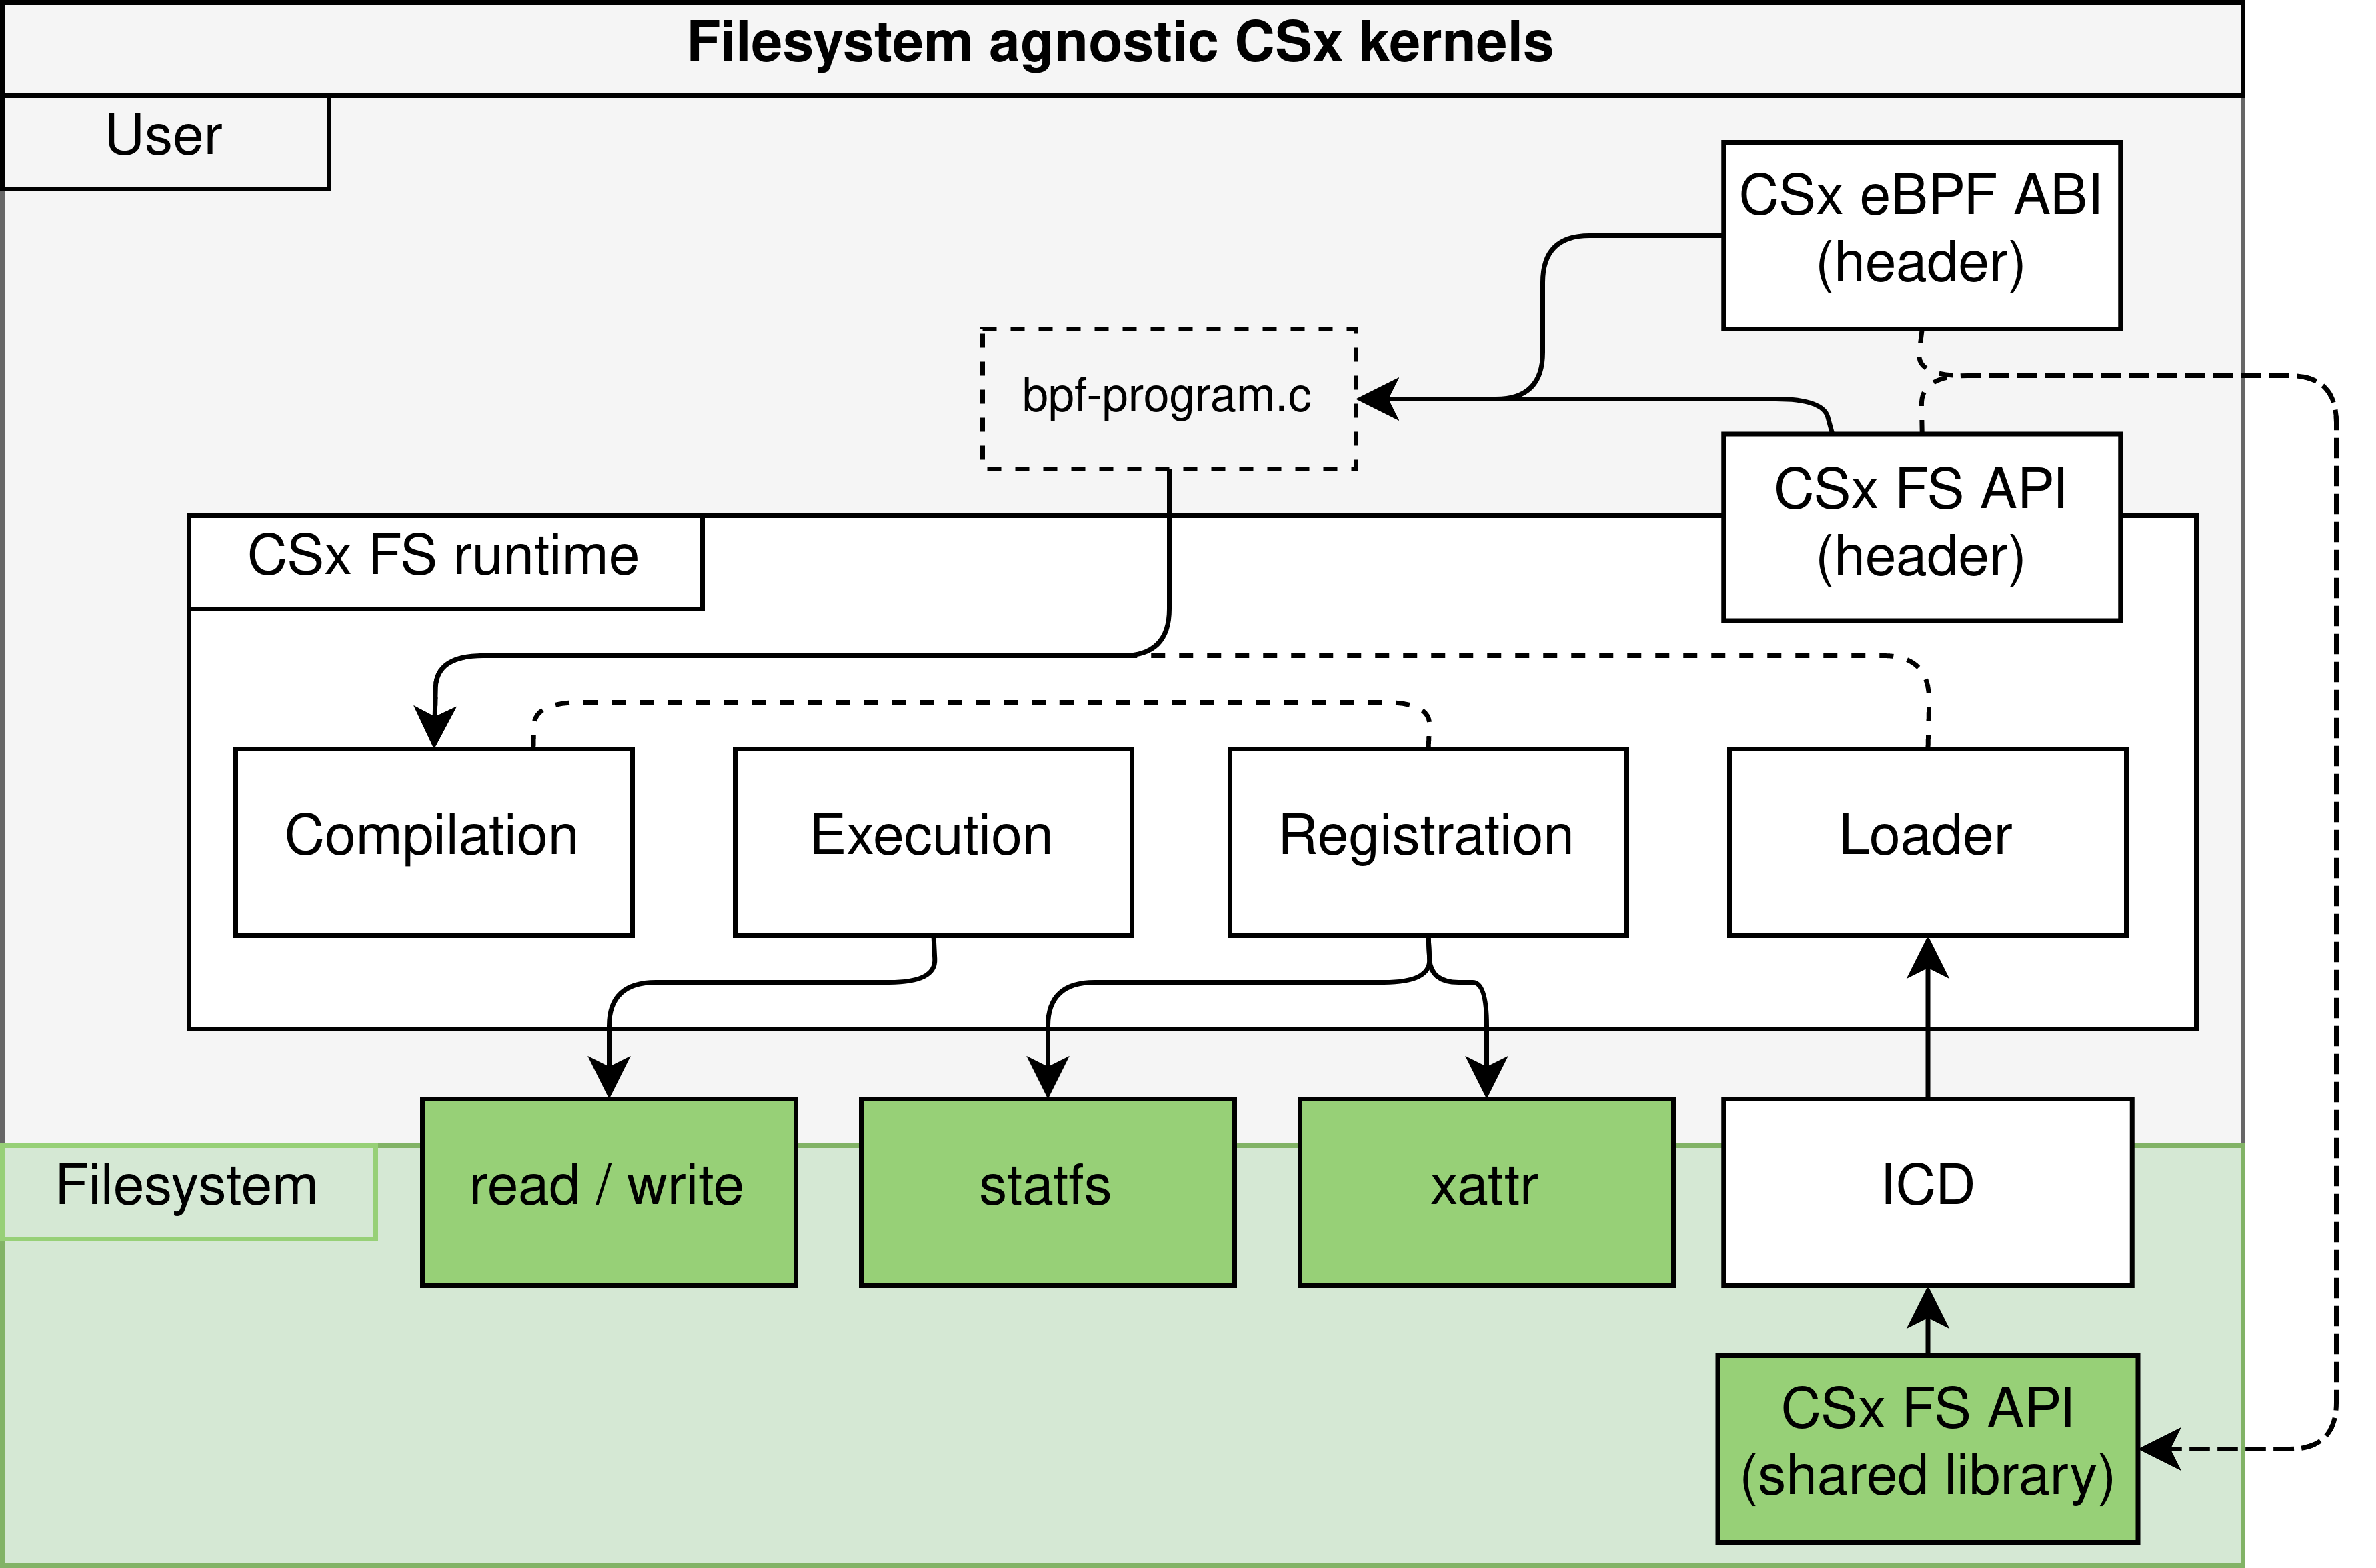
\includegraphics[width=0.7\textwidth]{resources/images/csx-fs-agnostic.png}
	\caption{Extended architecture to support filesystem agnostic CSx kernels.}
    % \includesvg[width=0.6\columnwidth]{resources/images/module-dependencies}
    \label{figure:csxfsruntime}
\end{figure}

Through this runtime the filesystem specific implementation of several
filesystem operations will be supplied. The required set of operations and
datastructures needs to be formalized and made part of the extension to NVMe
command set. Through the dynamic loading of shared libraries using a technique
from graphics APIs called \textit{Installable Client Drivers} (ICDs) the user
will not have to deal with recompilation. Such an ICD contains additional
metadata in a human readable markup language and can support extensions. The
CSx runtime can identify the filesystem and ICD for the current offloaded
operation through the use of \textit{statfs}. Furthermore, such a runtime can
provide host side scheduling mechanisms that are likely necessary in performant
multi-user tenancy applications.

% Use statfs to determine the type of filesystem, ICDs are related to a specific
% filesystem type. The CSx eBPF ABI should contain atleast one system call to
% retrieve the vendor filesystem context data for the current request (already
% part of prototype). The CSx FS API contains functions and datastructures to
% allow the kernel to transform this context data. The API is implemented by
% individual filesystems as shared library and made available throught the ICD.
% The CSx FS runtime uses a loader with mechanisms such as \textit{dlopen} to
% verify the contents of the provided library in accordance to the API.

% The basic format of the ICD can be extended such that it could support
% extensions to the base API as well as contain versioning. Typically, ICD files
% are human readable using a markup language such as YAML. This is same approach
% as the prominent video graphics API Vulkan.

\section{Kernel Safety}

The last consideration proposes mechanisms to ensure the execution of user
submitted code occurs safely. In the context of a filesystem this includes
preventing modifications to other files or regions of files. Additionally, it
requires preventing that an user submitted kernels reads regions of files it
should not have access to.

A potential first line of defence is the same system used by the Linux kernel
namely, static verification. Through static verification the Linux kernel
determines the behavior of an user submitted kernel prior to its execution.
However, to be able to determine the entire behavior statically many limitations
on how the kernel can be written need to be imposed. Particularly, loops with
bounds determined by parameters are problematic. This is because not only
false reporting of metadata, writes attributes to other files but also
termination can cause issues. A malicious user submitted kernel could
intentionally run an infinite loop, never terminating and consuming system
resources. To implement such a static verification system for eBPF existing
open-source tools such as ebpf-verifer \cite{ebpf-verifier} can be used.

Beyond static analysis the CSx can perform metadata and instrumentation that
reports about the behavior the kernel exhibited. Since each time an operation of
the ABI is called the uBPF VM traps into vendor code there would be no effective
mechanism for the user submitted kernel to hide this activity. Potentially, the
CSx could even immediatelly terminate the user submitted kernel without
executing the requested operation entirely. Granted the more flexible user
submitted kernels become the harder it becomes to identify malicious behavior.
Luckily the currently proposed stream and event kernels both would limit
malicious behavior to a single file. This is due to the append only nature of
ZNS devices as well as the absence of the \textit{reset} command from our ABI.

Lastly, the current implementation of uBPF can be extended such that the access
verifier can 

% How to ensure user submitted CSx compute kernels are safe?

% Potential mechanisms:
% - static verification
% - CSD instrumentation / metadata (report read / write operations and locations)
% - access verifier (runtime verification)

% ---------------------------------------------------------------------------
% ----------------------- end of thesis sub-document ------------------------
% ---------------------------------------------------------------------------